\documentclass[11pt,a4paper]{article}
\usepackage[utf8]{inputenc}
\usepackage[margin=2cm,top=1.9cm,bottom=2.1cm]{geometry}
\usepackage[expansion=false]{microtype}
\usepackage{graphicx}
\usepackage{booktabs}
\usepackage{amsmath,amssymb}
\usepackage{enumitem}
\usepackage[font=small,labelfont=bf,skip=3pt]{caption}
\usepackage{xcolor}
\usepackage[colorlinks=true,linkcolor=black,citecolor=black,urlcolor={rgb:red,0.1;green,0.35;blue,0.7}]{hyperref}
\usepackage{titlesec}
\titleformat{\section}{\large\bfseries}{\thesection}{0.6em}{}
\titlespacing*{\section}{0pt}{9pt}{4pt}
\titleformat{\subsection}{\normalsize\bfseries}{\thesubsection}{0.5em}{}
\titlespacing*{\subsection}{0pt}{6pt}{2pt}
\setlist{nosep,leftmargin=1.3em,topsep=2pt}
\setlist[itemize]{label=$\bullet$}
\setlength{\parskip}{3pt}
\setlength{\parindent}{0pt}
\setlength{\textfloatsep}{8pt}
\setlength{\floatsep}{6pt}
\renewcommand{\topfraction}{0.9}\renewcommand{\bottomfraction}{0.8}\renewcommand{\textfraction}{0.07}\renewcommand{\floatpagefraction}{0.85}
\setcounter{topnumber}{3}\setcounter{totalnumber}{5}
\DeclareTextSymbol{\textdollar}{OT1}{36}% dollar from cmr (avoids bitmap TS1 font)
\newcommand{\pct}{\%}
\makeatletter\let\tabinput\@@input\makeatother

\begin{document}

%======================================================================= COVER
\begin{titlepage}
\centering
\vspace*{2.2cm}
{\large Big Data, Machine Learning, with Applications to Economics and Finance\par}
\vspace{0.3cm}
{\normalsize Final project --- First submission (project proposal and data)\par}
\vspace{2.2cm}
\rule{\textwidth}{0.6pt}\par\vspace{0.5cm}
{\LARGE\bfseries Who Gets the Mortgage?\par}
\vspace{0.25cm}
{\Large Predicting and Explaining Home-Purchase Loan Denials\\ with 6.3 Million U.S.\ Applications (HMDA 2024--2025)\par}
\vspace{0.5cm}\rule{\textwidth}{0.6pt}\par
\vspace{2.2cm}
{\large\textbf{Author}\par}
\vspace{0.2cm}
{\large Vladimir Aristov\par}
\vspace{1.6cm}
{\normalsize Instructor: Fabián Slonimczyk\par}
\vspace{0.2cm}
{\normalsize International College of Economics and Finance, HSE University\par}
\vfill
{\normalsize September 30, 2026\par}
\end{titlepage}

%=============================================================== 1. INTRODUCTION
\section{Introduction}

Buying a home is the largest financial decision most households make, and the first
hurdle is getting the mortgage approved. In 2024 U.S.\ lenders denied roughly one in eleven
applications for a home-purchase mortgage. A denial comes late in the process, after the
applicant has chosen a home, paid application and appraisal fees and taken a hard
credit inquiry, and after the lender has spent underwriting resources on the file.
Denial rates also differ sharply across borrower groups, which makes mortgage denials a
long-standing question in the fair-lending literature
\cite{munnell1996,bartlett2022,fuster2022}.

\textbf{Objective.} The project builds a machine-learning system that, using only
information available when an application is submitted, predicts the probability that a
home-purchase mortgage application will be \emph{denied}. The data are the
\emph{universe} of loan-level records reported under the Home Mortgage Disclosure Act
(HMDA): 3.14 million applications in 2024 and 3.14 million in 2025. The project asks
four questions:
\begin{enumerate}[label=(\roman*)]
  \item \textbf{Prediction.} How well can denials be predicted out of sample, and out
  of \emph{time} (train on 2024, test on 2025), with interpretable versus flexible
  (ensemble) learners?
  \item \textbf{Explanation.} Which applicant, loan, lender and neighbourhood features
  drive predicted denials, and do model-based explanations agree with the denial
  reasons lenders actually report?
  \item \textbf{Fairness.} After conditioning on the financial profile the model sees,
  how much of the raw gap in denial rates across racial and ethnic groups remains?
  The model never uses protected attributes as inputs.
  \item \textbf{Economic value.} How much could a pre-screening tool save applicants
  (wasted fees, hard inquiries) and lenders (underwriting effort on files that will be
  denied), compared with simple rule-based cut-offs?
\end{enumerate}
Intended users: (a) applicants, brokers and fintech pre-qualification tools that
estimate approval odds before a costly application; (b) lenders triaging their
underwriting pipeline; (c) supervisors who need an ``expected-denial'' benchmark to
spot lenders whose decisions deviate from it.

%========================================================== 2. ML CLASSIFICATION
\section{The project within the machine-learning landscape}

\textbf{Classification of the task.}
\begin{itemize}
  \item \emph{Supervised learning.} Every record has a labelled outcome
  ($y=1$ if the application was denied, $y=0$ if it was approved).
  \item \emph{Binary classification with probability output.} What matters is a
  well-calibrated $\hat{P}(\text{denied}\mid x)$, not only a class label. The classes
  are \emph{imbalanced} (8.8\pct\ positives), so the planned metrics are ROC-AUC,
  precision--recall AUC and log-loss/Brier score, rather than accuracy. Decision
  thresholds will come from an explicit cost matrix.
  \item \emph{Structured (tabular) ``big'' data, batch (offline) learning.} There are
  6.3 million rows with a mix of continuous, ordinal and high-cardinality categorical
  features: 2{,}663 lenders and 418 metropolitan areas.
  \item \emph{Prediction and interpretation together.} The main target is out-of-sample
  prediction, but questions (ii)--(iii) also need interpretation: coefficients, partial
  dependence, SHAP values.
\end{itemize}

\textbf{Planned algorithms.} The models run from interpretable to flexible, following
the course \cite{islp}: logistic regression and lasso/ridge-penalised logit, LDA and naive Bayes,
a GAM with splines on DTI, LTV and income, and a pruned classification tree. The
flexible end has KNN (on a subsample), random forest, and gradient boosting
(XGBoost/LightGBM), with a stacked ensemble on top. Hyper-parameters are chosen by
stratified $k$-fold cross-validation on 2024. The 2025 file is an untouched
out-of-time hold-out.

\textbf{Why ML rather than a non-ML approach?} The alternatives are
(a) \emph{rule-based underwriting} with fixed cut-offs, and (b) the classic
\emph{econometric} approach: a hand-specified logit with linear terms, estimated in
sample to test one coefficient \cite{munnell1996}. ML has four advantages here:
\begin{enumerate}
  \item \emph{Non-linearities and interactions are learnt, not assumed.} Figure~\ref{fig:pred}a
  shows a U-shaped, sharply convex effect of DTI (denials jump from 5\pct\ to 80\pct\
  above a 60\pct\ DTI). Low-DTI files are denied \emph{more} often (11\pct), probably
  because they are low-documentation or non-standard files. A linear index misses
  this; trees and splines capture it. How DTI interacts with LTV, loan type and income
  (Fig.~\ref{fig:pred}c) is also hard to specify by hand.
  \item \emph{Model complexity is chosen by out-of-sample error, not in-sample
  fit.} Cross-validation and regularisation guard against over-fitting 2{,}663 lender
  effects. The 2025 hold-out measures how well the model survives a change of year.
  \item \emph{Better screening performance than rules.} A textbook rule ``deny if
  DTI\,$\geq$\,50\pct\ or LTV\,$>$\,100\pct'' flags 17\pct\ of applications but
  catches only 49\pct\ of denials, with 25\pct\ precision. Looser cut-offs
  (DTI\,$>$\,43\pct\ or LTV\,$>$\,97\pct) catch 70\pct\ of denials but flag 48\pct\ of
  all files, at 13\pct\ precision. A probabilistic model traces out the whole
  precision--recall frontier and can be tuned to the cost of each type of error.
  \item \emph{Scale.} Millions of rows and high-cardinality categoricals are where
  flexible learners gain most. The cost is interpretability, handled by comparing
  interpretable and black-box models and by post-hoc explanation tools.
\end{enumerate}

\textbf{Beyond the basics (what goes further than the lectures and seminars).}
\begin{itemize}
  \item \emph{Real big data and an out-of-time test.} The full national population of
  applications is used, not a toy sample. Validation is \emph{temporal}
  (2024\,$\rightarrow$\,2025), not only a random split, so the results speak to deployment.
  \item \emph{Leakage audit.} HMDA contains many fields that are filled in only
  \emph{after} a decision (Section~\ref{sec:leak}). Identifying and removing them is a
  substantive part of the design.
  \item \emph{High-cardinality categoricals.} Lender and MSA identities will be
  handled with out-of-fold target encoding and CatBoost-style ordered encoding, and
  compared with dropping them.
  \item \emph{Explainability tools not covered in class.} SHAP values
  \cite{lundberg2017}, compared against the lender-reported principal denial reason.
  This mirrors the ``adverse-action reason'' notices U.S.\ lenders must give under
  the Equal Credit Opportunity Act.
  \item \emph{Cost-sensitive evaluation and calibration} (Platt/isotonic) to value
  the system economically.
  \item \emph{Algorithmic-fairness audit.} Group calibration, and the gap in
  denial rates across groups that remains conditional on the model's prediction,
  following \cite{fuster2022}. Race, ethnicity and sex are excluded from the
  features. Because neighbourhood variables (e.g.\ tract minority share) can act as
  proxies, models will be compared with and without them.
\end{itemize}

%==================================================================== 3. DATA
\section{Data}

\subsection{Source and how the data are collected}
The data are the public \emph{modified Loan/Application Register} (LAR) files published
under HMDA (1975), implemented by the CFPB's Regulation~C (12~CFR~1003). Every covered
lender must record each mortgage application it receives and its outcome, and submit
the register to the CFPB/FFIEC by March~1 of the following year. Covered lenders are
banks and credit unions above an asset threshold with an office in a metropolitan area,
and non-bank lenders, that originated at least 25 closed-end mortgages in each of the two
preceding years. About 4{,}900 institutions reported 2024 data and 4{,}800 reported 2025
data. Submissions pass automated validity and quality edits before release. The public files are ``modified'' for privacy: loan amounts and property values
are rounded to the mid-point of \$10{,}000 bands, age is reported in bands, DTI is
binned outside 36--49\pct, and credit scores are withheld. The data were downloaded in
full from the FFIEC HMDA Data Browser API
(\url{https://ffiec.cfpb.gov/data-browser/}). It is also catalogued on Data.gov (``HMDA Public Data, starting in 2017'').

\textbf{Sample definition (fixed before any modelling).} The raw files hold 4.32m (2024)
and 4.36m (2025) home-purchase applications that ended in a decision:
originated, approved but not accepted, or denied. The sample keeps first-lien,
closed-end loans for a principal residence on a site-built one-to-four-unit home, and
excludes reverse mortgages and business-purpose loans. This leaves
\textbf{3{,}140{,}857} applications in 2024 and \textbf{3{,}139{,}327} in 2025.
Withdrawn and incomplete-file applications, and bare pre-approval requests, are
excluded because no credit decision on the merits was made.

\textbf{Dependent variable.} $y=\mathbf{1}\{\text{action taken}=\text{denied}\}$.
``Approved but not accepted'' counts as approved, since the lender said yes. The
denial rate is 8.81\pct\ in 2024 and 8.67\pct\ in 2025 (Fig.~\ref{fig:target}a).
Debt-to-income is by far the most common principal denial reason (38\pct), followed
by collateral (16\pct) and credit history (13\pct) (Fig.~\ref{fig:target}b).

\begin{figure}[!htbp]
\centering
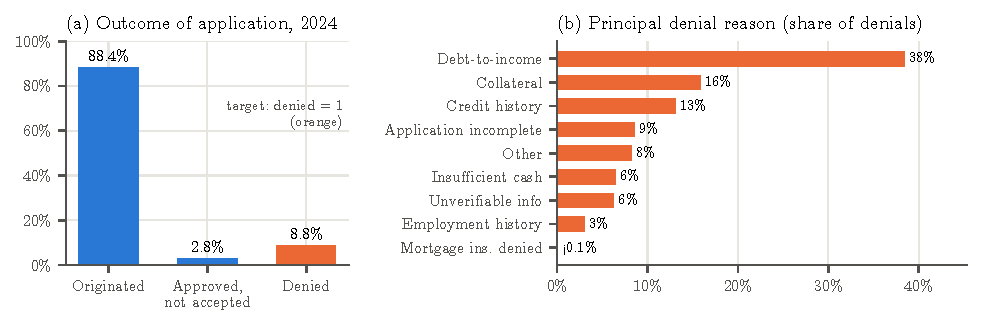
\includegraphics[width=\textwidth]{../../figs/fig1_target.pdf}
\caption{Dependent variable, 2024 sample ($N=3{,}140{,}857$). (a) Outcome shares.
(b) Lender-reported principal denial reason (description and validation only, never a feature).}
\label{fig:target}
\end{figure}

\subsection{Features and the leakage audit}\label{sec:leak}
\textbf{Candidate features} are those observable when the application is filed:
\begin{itemize}
  \item \emph{Loan:} amount, type (conventional/FHA/VA/USDA), term, ARM teaser
  period, interest-only and balloon flags, conforming-limit status.
  \item \emph{Applicant:} income, DTI, combined LTV, property value, age band,
  presence of a co-applicant, the credit-score model used.
  \item \emph{Process:} application channel (direct or via broker), the automated
  underwriting system used (Fannie Mae DU, Freddie Mac LPA, FHA TOTAL\ldots), lender
  identity.
  \item \emph{Location:} state, MSA, and census-tract minority share, relative
  income, housing age and owner-occupancy.
\end{itemize}

\textbf{Excluded because of leakage:}
\begin{itemize}
  \item \emph{Fields reported only for approved loans:} interest rate, rate spread,
  loan costs, points, lender credits, HOEPA status, purchaser type.
  \item \emph{The denial reasons themselves.}
  \item \emph{Two fields that turn out to encode the outcome.} Among applications
  flagged as pre-approval requests, the denial rate is exactly 0\pct\ (171k files):
  denied pre-approvals are recorded under a separate action code. The
  ``initially payable to institution = N/A'' category has an 84\pct\ denial rate,
  because lenders use it for loans that were never made.
\end{itemize}
Race, ethnicity and sex are kept \emph{only} for the fairness audit.

\subsection{Descriptive statistics}
Table~\ref{tab:num} summarises the continuous variables. The medians are plausible:
a \$325k loan and \$111k of income. The extreme tails show clear keying errors
(e.g.\ LTVs in the billions, incomes of \$7bn), so raw means and standard deviations
are meaningless here. The second submission will winsorise these values and use
robust transformations (logs, ratios). Missingness is low (below 3.1\pct) but not
random. Denied files are more often missing LTV and property value, and a missing DTI
carries a 34\pct\ denial rate. Missingness will therefore be encoded explicitly
rather than imputed silently.

\begin{table}[!htbp]
\centering\small
\caption{Continuous variables, 2024 sample (percentiles instead of mean/SD because of extreme outliers).}
\label{tab:num}
\begin{tabular}{@{}lrrrrrrrrr@{}}
\toprule
 & P1 & P10 & Median & P90 & P99 & Max & Miss.\,\% & \multicolumn{2}{c}{Median if\ldots} \\
\cmidrule(l){9-10}
 & & & & & & & & approved & denied \\
\midrule
\tabinput ../../results/table1.tex 
\bottomrule
\end{tabular}
\end{table}

Denied applicants have lower incomes (median \$86k versus \$114k), higher LTVs
(95\pct\ versus 90\pct) and higher loan-to-income ratios. They also live in tracts
with a higher minority share and lower relative income (Table~\ref{tab:num},
Fig.~\ref{fig:dist}a--b). Table~\ref{tab:cat} and Figure~\ref{fig:pred} show the
most informative categorical patterns:
\begin{itemize}
  \item \emph{Loan type.} Denial rates are higher for government-insured FHA loans
  (12.5\pct) than for conventional loans (7.6\pct).
  \item \emph{DTI} has the strongly non-linear effect described in Section~2
  (Fig.~\ref{fig:pred}a).
  \item \emph{LTV.} Denial rates are flat up to 100\pct\ LTV, then jump to over
  50\pct\ above 105\pct\ (Fig.~\ref{fig:pred}b).
  \item \emph{Income and loan type interact.} The FHA penalty is largest at the bottom
  of the income distribution, and the relation turns back up in the top decile
  (Fig.~\ref{fig:pred}c).
  \item \emph{Lenders differ a lot.} Among the 684 lenders with at least 500
  applications (93\pct\ of the sample), the 10th and 90th percentiles of the denial
  rate are 1.9\pct\ and 15.6\pct\ (Fig.~\ref{fig:pred}d). Lender identity is
  therefore a key feature, and a natural object for supervisory benchmarking.
  \item \emph{Race.} Raw denial rates range from 7.4\pct\ for White to 16.3\pct\ for
  Black applicants (Fig.~\ref{fig:dist}c). How much of this gap the financial
  variables explain is question~(iii).
\end{itemize}

\begin{table}[!htbp]
\centering\small
\caption{Selected categorical features, 2024 sample: share of applications and denial rate (\%).}
\label{tab:cat}
\begin{tabular}[t]{@{}llrr@{}}
\toprule
Feature & Level & Share & Denial \\
\midrule
\tabinput ../../results/table2a.tex
\bottomrule
\end{tabular}\hspace{1.2em}%
\begin{tabular}[t]{@{}llrr@{}}
\toprule
Feature & Level & Share & Denial \\
\midrule
\tabinput ../../results/table2b.tex
\bottomrule
\end{tabular}
\end{table}

\begin{figure}[!htbp]
\centering
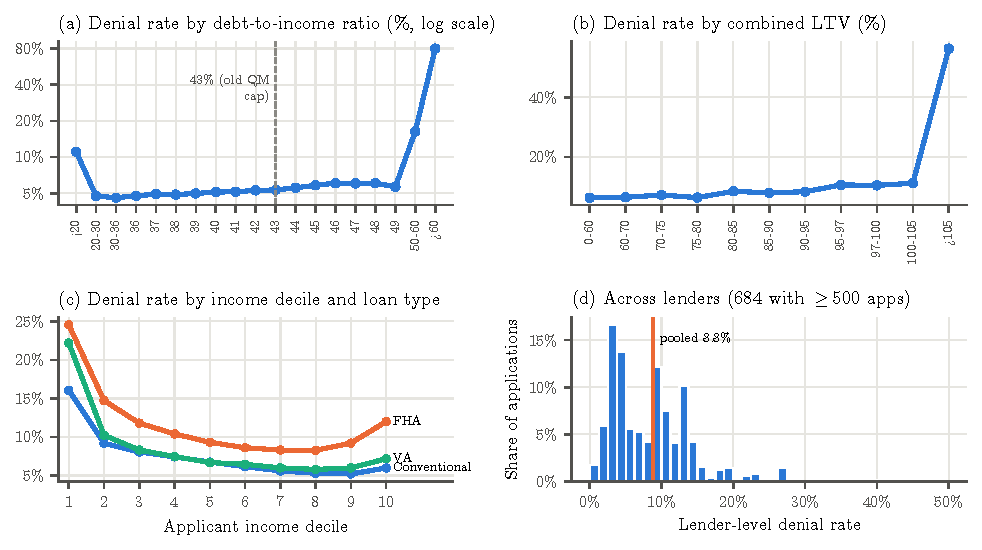
\includegraphics[width=\textwidth]{../../figs/fig2_predictors.pdf}
\caption{Denial rate against the main predictors, 2024. (a) DTI (log scale; bins
as reported in the public data). (b) Combined loan-to-value. (c) Income decile by loan
type. (d) Distribution of lender-level denial rates, weighted by applications.}
\label{fig:pred}
\end{figure}

\begin{figure}[!htbp]
\centering
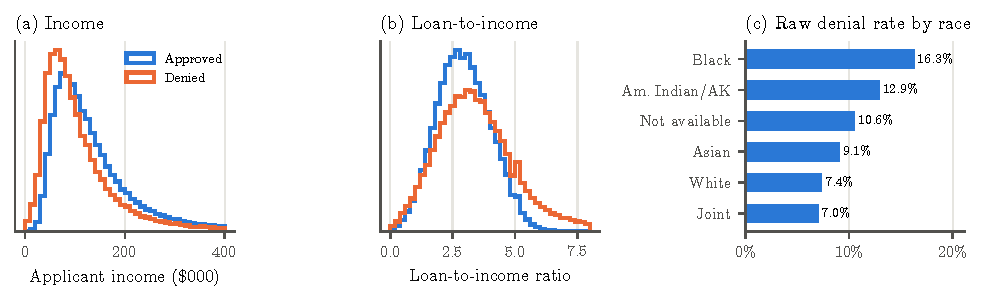
\includegraphics[width=\textwidth]{../../figs/fig3_distributions.pdf}
\caption{(a)--(b) Distributions of income and loan-to-income for approved and denied
applications (densities, truncated at the 99th percentile). (c) Raw denial rate by
applicant race, before any conditioning. Race is used only for the fairness audit.}
\label{fig:dist}
\end{figure}

\subsection{Representativeness and limitations}
The data are close to a census of U.S.\ mortgage applications rather than a sample.
Nearly all lenders of any size must report, the fields are standardised by
regulation, and the files are validated by regulators. A model trained on them should
therefore give reasonable answers for the U.S.\ market it would be deployed on.
The denial rate barely moves between 2024 and 2025 (8.81\pct\ versus 8.67\pct), and
the 2025 file tests temporal robustness directly. The main limitations are:
\begin{itemize}
  \item \emph{Missing variables.} Credit scores, assets and the AUS recommendation
  are not public. This caps accuracy, and part of any group gap may reflect them.
  \item \emph{Selection into applying.} Discouraged borrowers and withdrawn
  applications are not in the sample, so the model predicts denial \emph{conditional
  on reaching a decision}.
  \item \emph{The label is the lender's decision, not the borrower's later default.}
  The model learns underwriting practice, including any bias in it, which is exactly
  why the fairness audit matters.
  \item \emph{A high-rate period.} Results may shift in a different rate environment.
\end{itemize}

%========================================================================= END
\vspace{2pt}
\textbf{Code and reproducibility.} All code is submitted separately:
\texttt{01\_build\_sample.py} downloads and filters the data and
\texttt{02\_eda.py} produces every table and figure in this report. The notebook
\texttt{HMDA\_first\_submission.ipynb} runs the whole pipeline end to end.

\vspace{-4pt}
\begin{thebibliography}{9}\footnotesize
\setlength{\itemsep}{-1pt}
\bibitem{bartlett2022} Bartlett, R., Morse, A., Stanton, R., Wallace, N. (2022).
Consumer-lending discrimination in the FinTech era. \emph{Journal of Financial
Economics}, 143(1), 30--56.
\bibitem{fuster2022} Fuster, A., Goldsmith-Pinkham, P., Ramadorai, T., Walther, A.
(2022). Predictably unequal? The effects of machine learning on credit markets.
\emph{Journal of Finance}, 77(1), 5--47.
\bibitem{islp} James, G., Witten, D., Hastie, T., Tibshirani, R., Taylor, J. (2023).
\emph{An Introduction to Statistical Learning with Applications in Python}. Springer.
\bibitem{lundberg2017} Lundberg, S., Lee, S.-I. (2017). A unified approach to
interpreting model predictions. \emph{NeurIPS} 30.
\bibitem{munnell1996} Munnell, A., Tootell, G., Browne, L., McEneaney, J. (1996).
Mortgage lending in Boston: Interpreting HMDA data. \emph{American Economic Review},
86(1), 25--53.
\bibitem{cfpb} CFPB/FFIEC. HMDA Data Browser and Filing Instructions Guide (2024, 2025).
\url{https://ffiec.cfpb.gov/}.
\end{thebibliography}

\end{document}
